\documentclass{article}
\usepackage[utf8]{inputenc}
\usepackage[czech]{babel}
\usepackage{graphicx}
\clubpenalty=1000
\widowpenalty=1000
\hyphenpenalty=500
\tolerance=3000

\title{MoToX - programátorská dokumentace}
\author{Kateřina Nevolová \\ \texttt{katka.nevolova@gmail.com} \\ 73502469}

\begin{document}
\maketitle

MoToX je jednoduchá hra pro linux napsaná v jazyce C++ za pomocí knihoven GLUT
a OpenGL pro grafiku. Program se sestává z několika modulů, z nichž se většina stará o nějaký konkretní subsystém. Veškeré napojení na GLUT a hlavní cyklus programu je popsán v modulu main, který se dále odkazuje na game obstarávající herní
logiku. Většina modulů pak sdílí společný formát:

\begin{itemize}
\item inicializační a deinicializační funkci
\item funkci pro posun herního stavu o nějaký časový úsek
\item případně funkci pro vykreslení pomocí OpenGL
\item lokální data uložená v globální proměnné, většinou nějakém kontejneru
\end{itemize}

\section{Soupis modulů}

\subsection{main.cpp}
Obsahuje funkci main s GLUTovými funkcemi pro vytvoření a obsluhování
OpenGL okna apod., sbírá a pamatuje si klávesnicový vstup. Snímá
přesný čas hry a předává ho dál herní logice do modulu game.
Periodicky vyvolává překreslení scény.

\subsection{game.cpp}
Inicializuje (a při vyvolání nového levelu resetuje) všechny součásti hry. Pamatuje si čas a status hry a zvolenou mapu. Funkcí \texttt{init\_map} komunikuje s modulem maplist funkcí \texttt{maplist\_get\_file\_name}, podle vybraného mapového souboru potom načte level funkcí \texttt{read\_map\_file}.
Funkce \texttt{draw\_game} kreslí celou hru a je přepínána podle statusu hry (hráč je právě v menu, ve hře, vyhrál, či prohrál). Dále komunikuje s modulem text funkcemi \texttt{draw\_string} a \texttt{text\_length} pro výpis statistik a jiného textu hry a jeho pohodlné zarovnávání. Funkce \texttt{update\_game} posune
všechny herní součásti o specifický časový interval a zpracovává
klávesnicový vstup z modulu main. Udržuje souřadnice kamery (hráč je stále ve středu hracího pole). V případě hráčovy smrti (\texttt{moto\_out\_of\_map}, \texttt{moto\_touches\_enemy} - funkce z modulu moto) či vítězství (funkce \texttt{enemies\_left} - funkce z modulu enemy) dává možnost spustit hru znovu, nebo se hrou dobrovolně skončit.

\subsection{moto.cpp}
Modul moto se stará o samotnou motorku, kreslí ji (funkce \texttt{draw\_moto}) a udržuje parametry jejích kol a hlav. Funkce \texttt{update\_moto} slouží k ovládání samotného stroje, je volána z modulu game a zpracovává konečný klávesnicový vstup. Pomáhá si funkcí \texttt{rotate} (odtud) a \texttt{spring} (z modulu ball) pro snadnější vybalancovávání a soudržnost kol a řeší kolize kol s okolím funkcí z map.cpp \texttt{collide\_ball\_with\_walls}. Komunikuje s modulem bullets funkcí \texttt{add\_bullet}.
Funkce \texttt{get\_moto\_position} a \texttt{moto\_out\_of\_map} jsou volány opět z gamu a slouží pro účely kamery a pro kontrolu pozice motorky.
Funkce \texttt{moto\_touches\_enemy} zjišťuje pomocí funce z enemy.cpp \texttt{ball\_touches\_enemy} zda nedošlo ke kolizi s nepřáteli, popřípadě zavolá \texttt{big\_explosion} z modulu particles.

\subsection{enemy.cpp}
List \texttt{enemies} uchovává pozici, rychlost, životy a další
parametry nepřátel. Funkce \texttt{move\_enemies} posunuje nepřátele o časový tik, nechá je kolidovat s prostředím funkcí \texttt{collide\_ball\_with\_walls} a pokud je někdo z nepřátel mimo mapu, smaže ho. Funkce \texttt{draw\_enemies} nepřátele kreslí. Kolize se střelami hráče jsou ošetřovány funkcí \texttt{try\_to\_damage\_enemy}, která nalezne cíl a případně smaže nepřítele a udělá výbuch (\texttt{big\_exposion}) z particlů. Funkce \texttt{ball\_touches\_enemy} zjišťuje kolizi kolečka motorky a nepřátel (volána z modulu moto.cpp). Funkci \texttt{enemies\_left} používá modul game, aby zjistil, zda už hra neskončila vítězstvím.

\subsection{bullets.cpp}
Obhospodařuje list s pozicí, rychlostí a způsobovaným poškozením střel. Funkcí \texttt{update\_bullets} je updatuje, nechává vykreslovat (\texttt{add\_particle}), koliduje se stěnami funkcí \texttt{collide\_ball\_with\_walls} z modulu map, popřípadě nechá vyrobit \texttt{small\_explosion}. Maže střely pokud jsou pryč z mapy (\texttt{out\_of\_map}) nebo pokud zasáhly nepřítele (\texttt{try\_to\_damage\_enemy}).

\subsection{ball.cpp}
Modul ball se stará o hru na té nejnižsí úrovni. Funkcí \texttt{collision} (volanou z modulu map) se stará o kolizi kuličky s libovolnou přímkou - napomáhá si funkcí \texttt{normalize} a \texttt{wall\_collision}, která už konečně řeší veškeré přepočítání pozic a rychlostí při kolizích. Funkce \texttt{spring} volaná z modulu moto se stará o přitažlivost kuliček a pružení.

\subsection{map.cpp}
Modul map udržuje a vykresluje list stěn a překážek. Funkce \texttt{collide\_ball\_with\_walls} je volána téměř ze všech modulů hry a stará se po zavolání funkce \texttt{collision} z ball.cpp o kolize kola s mapou. Funkce \texttt{out\_of\_map} udržuje hranice mapy pro hru podobně jako funkce \texttt{map\_bottom}.

\subsection{maplist.cpp}
Tento modul inicializuje (funkcí \texttt{maplist\_init}) a spravuje adresář map, ověřuje zda jsou soubory v adresáři maps skutečně mapami (funkcí \texttt{process\_filename}) a pokud ano přidává je do vektoru map. Udržuje počet map. Funkcemi \texttt{maplist\_get\_name} a \texttt{maplist\_get\_file\_name} pomáhá modulu game pohodlně načítat požadované mapy a vykreslovat interface.

\subsection{particles.cpp}
Modul pro kreslení částicového systému (explozí apod.). Všechny
částice jsou uložené v listu, každá má
svoji pozici, rychlost (směr), barvu, trvanlivost a jeden ze tří
předem určených tvarů. Partikly jsou zde kresleny a updatovány. Různé moduly hry volají funkce \texttt{small\_explosion} a \texttt{big\_explosion} pro různé typy explozí.

\subsection{text.cpp}
Jednoduchý nástroj pro kreslení a zjištění délky textu, font je ručně poskládaný z vektorů.

\section{Kompilace a spuštění hry}

Ke kompilaci jsou potřeba knihovny GLUT a OpenGL. Program se sestaví pomocí
Makefile příkazem \texttt{make}. Skompilovaný program je poté připraven ke
spuštění příkazem \texttt{./motox}.

\section{Screenshot s popisem}
\begin{center}
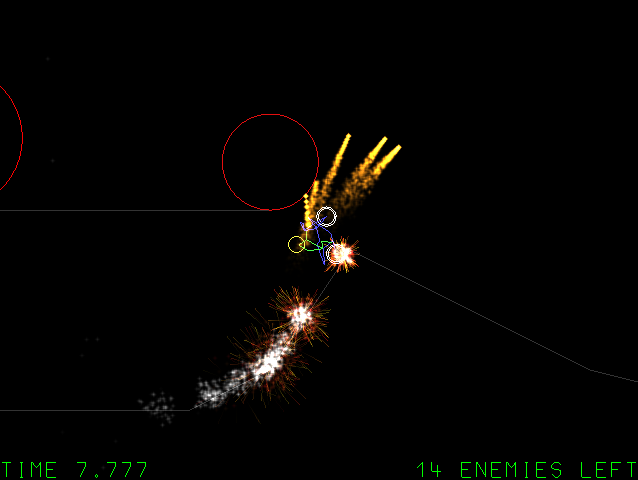
\includegraphics[width=10cm]{combat.png}
\end{center}

Motorku ovládáme šipkami, mezerníkem a klávesou \texttt{x}. Stroj vykresluje modul moto. Modul game pomocí fontů z modulu text kreslí informace o hře (čas hry a počet nepřátel, které je potřeba eliminovat) v dolní části okna. Výbuchy, kouř a střely obhospodařuje modul bullets a vykresluje modul particles. Šedé plošinky pochází z modulu map a kreslí je game. Nepřátelské objekty reprezentují červené kružnice, ke kterým není radno se přibližovat.

\end{document}
